\chapter{Heat Equation -- 2D -- Axi Symmetric Steady State Radiation}

\modinfo{Directory}{Radiation}
\modinfo{Solvers}{\Idx{HeatSolve}}
\modinfo{Tools}{\Idx{ElmerGUI}}
\modinfo{Dimensions}{2D, Axi-Symmetric}
\modinfo{Author}{Juha Ruokolainen, Rich Bayless}


\subsection*{Case definition}

At high temperature the radiation heat transfer between walls 
is often the dominating heat transfer mechanism. In this
tutorial we examine how radiation heat transfer between 
concentric cylinders is modelled.\\

The problem is a pure heat transfer problem that may be solved
with \texttt{HeatSolve}. The view and Gebhart factors 
associated with the radiation are solved as a first step 
in solving the equations. Thereafter the non-linear heat equation 
is solved until convergence is reached.


\begin{figure}
\begin{center}
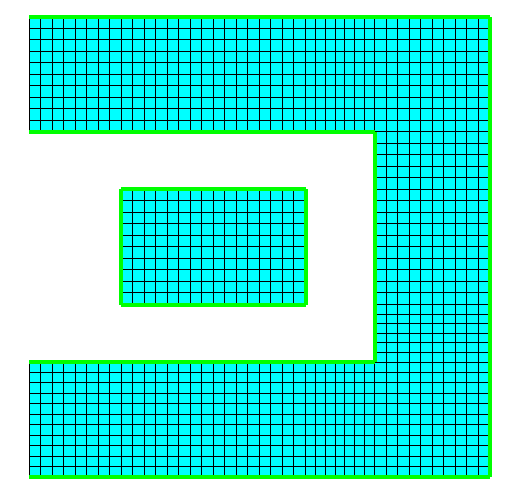
\includegraphics[width=100 mm]{geometry}
\caption{Geometry and mesh}\label{fg:geometry}
\end{center}
\end{figure}  


\subsection*{Solution procedure}

The mesh is given in ElmerGrid format in file \texttt{radiation.grd}, load this file.
\ttbegin
File 
  Open -> radiation.grd
\ttend
You should obtain your mesh and may check \texttt{Model Summary...} that 
it consists of 1231 surface elements.  Your geometry and mesh should look something
like as shown in figure \ref{fg:geometry}\\


After we have the mesh we start to go through the Model menu from the top to bottom. 
In the Setup we choose things related to the whole simulation such as file names, 
time stepping, constants etc.  

The simulation is carried out in Axi Symmetric coordinates. The only constant 
required is the Stefan-Boltzmann constant that gives the
relationship between temperature and radiation power, and this
constant is predefined in the \texttt{Setup} menu.

\ttbegin
Model
  Setup 
     Coordinate System = Axi Symmetric
     Simulation Type = Steady State
     Steady State Max Iterations = 1
     Output Intervals = 1
  Apply
\ttend
In the equation section we choose the relevant equations and parameters related to their solution. 
In this case we'll have the Heat equation.

When defining Equations and Materials it is possible to assign to the bodies 
immediately, or to use mouse selection to assign them later. In this case we 
have just two bodies and therefore its easier to assign the Equation and 
Material to it directly.

For the linear system solvers we are happy to use the defaults. One may however, try out different
preconditioners (ILU1,\ldots) or direct Umfpack solver, for example.
\ttbegin
Model
  Equation
   Name = Radiation
    Apply to Bodies = 1 2
    Heat Equation
      Active = on
    Edit Solver Settings
       Steady State
         Convergence Tolerance = 1.0e-8
       Non-linear system
        Convergence Tolerance = 1.0e-8
        Max Iterations = 50
        Relaxation Factor = 0.7
        Newton After Iterations = 1
        Newton After Tolerance = 1.0e-4
      Linear system
        Convergence Tolerance = 1.0e-12
        Preconditioning = ILU1
    Add 
    OK
\ttend        
The Material section includes all the material parameters. They are divided into 
generic parameters which are direct properties of the material without making 
any assumptions on the physical model, such as the mass. Other properties 
assume a physical law, such as conductivities and viscosity. 

The material properties differ only in heat conductivity. Heat capacity is not
actually needed since the case is not transient. The inner body has ten times
higher conductivity than the outer body.

\ttbegin
Model
  Material
    Name = Inner
    Apply to Bodies = 1 
    General 
      Density = 1.0
      Heat capacity = 1.0
    Heat Equation
      Heat Conductivity = 10.0
    Add
    New

    Name = Outer
    Apply to Bodies = 2 
    General 
      Density = 1.0
      Heat capacity = 1.0
    Heat Equation
      Heat Conductivity = 1.0
    Add
    OK
\ttend

A Body Force represents the right-hand-side of a equation. The body 
force is the heating power in units W/kg. 
 

\ttbegin
Model
  Body Force
    Name = Power
    Apply to Bodies = 1
    Heat Equation
       Volume Heat Source = 10000
    Add 
    OK
\ttend    

Initial conditions are needed in this case. We choose a 
constant Temperature field of 250C. 
\ttbegin
Model
  Initial Condition 
    Name = Initial
    Apply to Bodies = 1 2
    Heat Equation
      Temperature = 250.0
    Add 
    OK
\ttend

Only one boundary condition may be applied to each boundary and therefore all the 
different physical BCs for a boundary should be grouped together. 

The radiation boundary conditions are set for two different boundaries. The first one
is for the internal heated object and the second one for the outer insulating body. 
The normal direction of the surfaces is important since a wrong direction may 
result to a badly set problem for the view factor computation. Internal and 
external surfaces are very different.  The normal direction may be switched 
with the input box \texttt{Radiation Target Body}. A good sign of a properly 
set case is that the view factors add up to about one.

The third boundary condition is the Dirichlet condition for the external boundary.
Dirichlet conditions boost up the convergence even though the heat equation 
is basically well defined also with external radiation conditions.
\ttbegin
Model
  BoundaryCondition
    Name = Inner
    Apply to Bodies = 1
    Heat Equation
      Radiation Settings = Diffuse Gray
      Emissivity = 0.6
      Radiation Target Body = -1
    Add
    New

    Name = Outer
    Apply to Bodies = 2
    Heat Equation
      Radiation Settings = Diffuse Gray
      Emissivity = 0.1
      Radiation Target Body = -1
    Add 
    New

    Name = Exterior
    Apply to Bodies = 3
    Heat Equation
      Temperature = 100.0
    Add 
    OK
\ttend   

The conditions may also be assigned to boundaries in the Boundary condition menu, or 
by clicking with the mouse. Here we use the latter approach as that spares us of the 
need to know the indexes of each boundary.
\ttbegin
Model
  Set boundary properties
   Choose Inner -> set boundary condition Inner
   Choose Outer -> set boundary condition Outer
   Choose Exterior -> set boundary condition Exterior
  Update
\ttend


For the execution ElmerSolver needs the mesh files and the command file. 
We have now basically defined all the information for ElmerGUI to write the 
command file. After writing it we may also visually inspect the command file.
\ttbegin
Sif 
  Generate
  Edit -> look how your command file came out  
\ttend

Before we can execute the solver we should save the files in a directory. 
The ElmerGUI project includes all the files needed to restart the case.
\ttbegin
File 
  Save Project
\ttend

After we have successfully saved the files we may start the solver
\ttbegin
Run
  Start solver
\ttend
A convergence view automatically pops up showing relative changes of each iteration.

When there are some results to view we may start the postprocessor also
\ttbegin
Run
  Start ParaView
\ttend

\subsection*{Results}

With the given computational mesh the problem is solved in 
a few seconds. With 1,231 second order 9-noded
rectangular elements the maximum temperature is 565.7~K.
The corresponding results are shown in Fig.~\ref{fig:temp_rad1}.

\begin{figure}
\begin{center}
  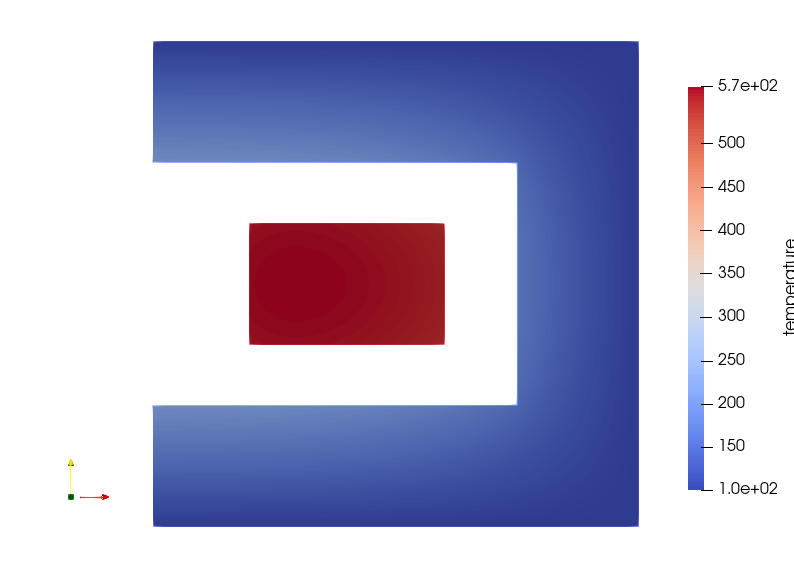
\includegraphics[width=100mm]{temp_rad1}
\end{center}
\caption{Temperature distribution in the radiation heat transfer
problem}
\label{fig:temp_rad1}
\end{figure}
 



\hfill
